\section{Automatisierung von Geschäftsprozessen}\label{sec:Automatisierung}
Über Geschäftsprozesse lässt sich die Unternehmensstrategie mit den unterstützenden Informations- und Anwendungssystemen verknüpfen.
In einem wirkungsvollen Unternehmensmanagement müssen demnach diese drei Ebenen der Strategie, der Geschäftsprozesse und der \ac{IT} in ihrer Gesamtheit berücksichtigt werden.
\cite{Scheer.1991}
Insbesondere bei der \ac{IT}-Unterstützung der operativen Geschäftsprozessausführung auf der unteren Ebene ist es vorteilhaft, die Diskrepanzen zwischen den tatsächlichen Geschäftsprozessen und deren informationstechnischen Repräsentation möglichst gering zu halten.
\cite{Gadatsch.2013}

Der Einsatz von Verfahren zur geschäftsprozessorientierten Systemgestaltung wird als adäquates Mittel zur Verknüpfung der betriebswirtschaftlichen mit der informationstechnischen Perspektive angesehen, da derart Verfahren durch semiformale Notationsweisen sowohl komplexe Sachverhalte der Betriebswirtschaft systematisch unterstützten als auch die notwendige Genauigkeit für den Entwurf von Informationssystemen bieten.
\cite{Staud.2006}
Ein Geschäftsprozessmodell repräsentiert dabei im Allgemeinen eine Repräsentanz eines Ausschnittes der realen Welt, im konkreten Fall die Abbildung eines existenten Geschäftsprozesses, die entweder in Gestalt eines Ist-Modells die derzeitige Situation oder in der Ausprägung eines Soll-Modells eine potenziell angestrebte Möglichkeit darstellt.
\cite{Becker.2012}

Die Modellierung von Geschäftsprozessen verfolgt verschiedene Einsatzzwecke.
Dies betrifft zum einen die organisatorische Gestaltung, wie etwa die Dokumentation, Reorganisation oder Optimierung von strategischen und operativen Geschäftsprozessen. 
Auf der anderen Seite können durch das Zusammenfügen der betriebswirtschaftlichen mit der informationstechnischen Perspektive Kriterien für die Gestaltung von Informationssystemen bestimmt werden, welche für die Automatisierung von Geschäftsprozessen eine herausragende Rolle spielen.
\cite{Scheer.2017}
Unter der Automatisierung von Geschäftsprozessen wird in der vorliegenden Bachelorarbeit in Anlehnung an \citeauthor{Abolhassan.2016} \cite{Abolhassan.2016} sowie \citeauthor{Jobst.2010} \cite{Jobst.2010} die digitale Unterstützung und vollständige oder teilweise digitale Ausführung manueller Geschäftsprozesse verstanden.

Um ein Geschäftsprozessmodell letztlich in Gestalt eines Informationssystems abzubilden, existieren alternative Ansätze, wie etwa die Verwendung des Geschäftsprozessmodells zur Beschreibung von zugehörigen Anforderungen, um eine softwaretechnische Implementierung im Rahmen eines Anwendungssystems zu realisieren, die unternehmensspezifische Anpassung von Standardsoftware oder die Umsetzung in ausführbaren Modellen in geeigneten Ausführungsumgebungen.
\cite{Lehmann.2008} 
Im Rahmen dieser Bachelorarbeit wird lediglich der erste Ansatz in Betracht gezogen, demnach werden Anwendungssysteme als Aufgabenträger zur Automatisierung von Geschäftsprozessen verstanden, wohl wissend, dass nicht jeder Geschäftsprozess vollständig automatisierbar ist.

\subsection{Merkmale und Kriterien}
Der Einsatz von Verfahren zur geschäftsprozessorientierten Systemgestaltung bietet die Möglichkeit automatisierbare Geschäftsprozesse in fachlich sowie technisch spezifizierten Geschäftsprozessmodellen formalisiert und detailliert zu erfassen.
Grundsätzlich lässt sich die Gestaltung von Geschäftsprozessen dieser Art in einem kreisförmigen Lebenszyklusmodell zum Ausdruck bringen, das in die organisatorische Unternehmensgestaltung integriert werden muss. 
\cite{Scheer.1991}
Ein solches Modell beschreibt den sich wiederholenden, idealtypischen Ablauf der verschiedenen Aufgaben der Geschäftsprozessentwicklung und betont dadurch dessen kontinuierlichen Charakter gegenüber einmaligen und isolierten Prozessverbesserungsinitiativen.
\cite{Leiting.2012}

In der Literatur findet sich eine Vielzahl unterschiedlicher Lebenszyklusmodelle.
\cite{MacedodeMorais.2014} 
Diese unterscheiden sich zwar hintsichtlich der Anzahl, Benennung sowie Partitionierung der einzelnen Aufgaben in Lebenzyklusphasen, in ihrer Essenz weichen sie jedoch nicht fundamental voneinander ab.
\cite{Houy.2010}
In der vorliegenden Bachelorarbeit wird das etablierte Lebenszyklusmodell von \citeauthor{Scheer.1991}
\cite{Scheer.1991} zugrunde gelegt.
Der Ablauf dieses aus vier Phasen bestehenden Modells ist in Abbildung \ref{fig:Phasenmodell bei der Automatisierung von Geschäftsprozessen} illustriert und wird im Folgenden näher beleuchtet.

Im ersten Schritt wird eine \ac{IT}-orientierte fachliche Ausgangslösung erstellt.
Diese ergibt sich aus der eingehenden Analyse eines neuen oder existierenden Geschäftsprozesses, in Abbildung \ref{fig:Phasenmodell bei der Automatisierung von Geschäftsprozessen} im linken oberen Bereich veranschaulicht, durch die zunächst die grundsätzlichen Anforderungen des zu untersuchenden Geschäftsprozesses sichtbar gemacht werden.
\cite{Schwegmann.2002}
Aus diesem Grund werden hier auch noch alle Perspektiven zusammen betrachtet.

Die darauf folgende Konzeptionsphase behandelt, auf Basis der zuvor erhobenen Anforderungen an einen Geschäftsprozess, dessen Beschreibung auf fachlicher Ebene. 
\cite{Schwegmann.2002}
Anschließend wird das Fachkonzept, unabhängig von Implementierungsgesichtspunkten, mit technischen Anforderungen an das Anwendungssystem angereichert, sodass es als Ausgangspunkt für eine konsistente softwaretechnische Implementierung dienen kann.
\cite{Scheer.1991}
Dabei wird jedoch noch kein Bezug zu plattformspezifischen Programmiersprachen hergestellt. 
Das technisch spezifizierte Konzept kann geändert werden, ohne dass dies Auswirkungen auf das Fachkonzept hat.
\cite{Speck.2002}
Dies bedeutet jedoch nicht, dass Fachkonzept und technische Spezifikation isoliert voneinander entwickelt werden können. 
Mehr noch soll nach Abschluss der fachkonzeptionellen Darstellung der betriebswirtschaftliche Inhalt so definiert sein, dass ausschließlich \ac{IT}-bezogene Argumente, wie das Leistungsverhalten eines Informationssystems, keine Auswirkungen auf die Fachinhalte nehmen können.  

\begin{figure}[H]
	\centering 
    \begin{tikzpicture}
       \arcarrow{177}{ 96}{Analyse}
       \arcarrow{ 89}{  3}{Konzeption}
       \arcarrow{268}{361}{Implementierung}
       \arcarrow{179}{271}{Ausf{\"u}hrung}
    \end{tikzpicture}
    \caption[Phasenmodell bei der Automatisierung von Geschäftsprozessen]
    {Phasenmodell des Lebenszyklus von Geschäftsprozessen \protect\footnotemark}
    \label{fig:Phasenmodell bei der Automatisierung von Geschäftsprozessen}
\end{figure}
\footnotetext{Eigene Darstellung, in Anlehnung an \citeauthor{Scheer.1991} \citeyear{Scheer.1991} \cite{Scheer.1991} }

In der Implementierungsphase wird das Geschäftsprozessmodell in eine ausführbare Programmiersprache überführt somit in eine Anwendungssoftware transformiert, getestet und in ein Anwendungssystem integriert.
\cite{Scheer.1991}
Während der Ausführungsphase erfolgt häufig eine Überwachung des laufenden Geschäftsprozesses, um in einer nachfolgenden Iteration des gesamten Phasenmodells eine Optimierung des Geschäftsprozessmodells basierend auf den angeeigneten Erkenntnissen durchführen zu können.
\cite{Scheer.2005}
Der Fokus dieser Bachelorarbeit liegt insbesondere auf der Phase der Analyse bis zur softwaretechnischen Implementierung, wohingegen die Ausführung vernachlässigt wird.

In der geschäftsprozessorientierten Systementwicklung steht während der Modellierung die ablauforientierte Sicht im Mittelpunkt.
Geschäftsprozessorientierte Modellierungsansätze betrachten das darzustellende Informationssystem ausgehend von der der informationstechnischen Unterstützung menschlicher Arbeitsabläufe, die sie erfüllen sollen, und dem dazu notwendigen Vorgehen, das sich aus der Folge der durchzuführenden Aktivitäten ergibt.
\cite{Wolf.2016}
Dabei werden die zu erfüllenden Aktivitäten systematisch analysiert und anschließend entsprechend ihrer Reihenfolge in den Geschäftsprozess integriert werden.
Eine Aktivität \footnote{Aktivitäten werden in anderer Literatur oft auch als Geschäftsprozessschritte bezeichnet.} ist ein diskreter Schritt innerhalb eines Prozesses, welcher entweder manuell durch einen Menschen oder automatisch durch einen Dienst durchgeführt wird.
\cite{Benker.2016}
Das daraus resultierende Geschäftsprozessmodell repräsentiert den zur Erfüllung der Aufgabe notwendigen Ablauf von Aktivitäten, mit welchem ein übergeordneter Geschäftszweck verfolgt wird.

Durch die stetige Verbreitung von serviceorientierten Architekturen besteht für Unternehmen die Möglichkeit, vollständige Geschäftsprozesse oder einzelne Aktivitäten auf Basis modularer digitaler Dienste in einer lose gekoppelten Weise aufeinander abzustimmen und zu automatisieren. 
\cite{Masak.2007}
Eine \ac{SOA} zielt auf eine optimale Unterstützung der fachlichen Geschäftsprozesse durch die Dynamisierung der Informationssysteme ab; Unternehmensstrategie und Informations- und Anwendungssysteme sollen besser integriert werden.
\cite{Teusch.2016}

% \interfootnotelinepenalty=10000
\begin{figure}[H]
	\centering 
    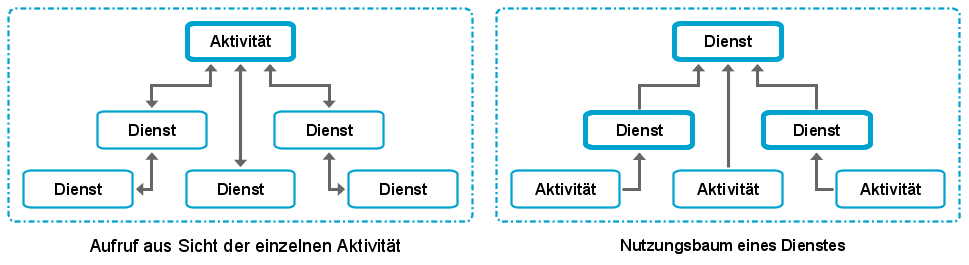
\includegraphics[width=\textwidth]{img/Serviceaufbau.png}	
    \caption[Nutzung eines Dienstes]
    {Nutzung eines Dienstes  \protect\footnotemark}
    \label{fig:Nutzung eines Dienstes}
\end{figure}
\footnotetext{Eigene Darstellung, in Anlehnung an \citeauthor{Masak.2007} \citeyear{Masak.2007} \cite{Masak.2007} }
\footnotetext{Die Abbildung dient lediglich der Visualisierung und ist nicht \acs{BPMN} 2.0 konform.}

Hierbei wird die wesentliche Geschäftslogik der Aktivitäten in digitalen Diensten gekapselt, während der übergreifende Geschäftsprozess in Form von Anwendungssoftware die eher reaktive und demnach dynamische Ausführungssemantik implementiert. 
\cite{Teusch.2016}
Unter dem Aspekt der Wiederverwendbarkeit eines Dienstes in einer \ac{SOA} sollte des Weiteren der in Abbildung \ref{fig:Nutzung eines Dienstes} illustrierte Umstand, dass digitale Dienste zur Ausführung einer Aktivität auf Basis weiterer Dienste aufgebaut sein können oder im Umkehrschluss ein Dienst von unterschiedlichen Aktivitäten genutzt werden kann, einer kritischen Betrachtung unterzogen werden.
\cite{Masak.2007}

Sogenannte Webservices stellen dabei eine auf \ac{XML} ausgerichtete und auf offenen Standards basierende Technologie zur Realisierung einer \ac{SOA} dar, indem sie die in einer beliebigen Programmiersprache implementierte Geschäftslogik in Form von Diensten anhand vereinheitlichter Schnittstellen nach außen zur Verfügung stellen.
\cite{Masak.2005}
An dieser Stelle sei jedoch der Hinweis erlaubt, dass das Konzept der Serviceorientierung allgemeiner ist und schon früher existierte als Webservices. Webservices sollten daher nur als eine, wenn auch nur zum Verfassungszeitpunkt dieser Bachelorarbeit als wahrscheinlich am besten geeignete Möglichkeit zur Realisierung serviceorientierter Architekturen betrachtet werden.

Ein Webservice ist als Maschine-zu-Machine-Kommunikation zu verstehen. Diese Maschinen sprechen über offenen Standards miteinander. 
\cite{Finger.2009b}
Nachdem ein Webservice in ein Anwendungssystem integriert wurde, erfolgt die Kommunikation in der Regel automatisch. 
Ein Endanwender auf der Seite der Benutzerschnittstelle wird nicht zur Kenntnis nehmen, dass die Anwendungssoftware, die er bedient, mit einem Webservice kommuniziert. Dieses Prinzip entspricht ebenfalls dem Grundgedanken einer \ac{SOA}.
\cite{Teusch.2016}
Auf diese Weise können Webservices beispielsweise aus einem Geschäftsprozess heraus aufgerufen werden, ohne ihre konkrete Implementierung zu kennen, was insbesondere in einem geschäftsprozess- oder unternehmensübergreifenden Kontext ein bedeutender Faktor ist. Zur Änderung eines Geschäftsprozesses bedarf es lediglich einer Anpassung der Ausführungssemantik der Anwendungssoftware durch veränderte Aufrufe von bestehenden oder zusätzlichen Webservices.

% \todo{SOA Texte durch SAP Book Quelle ersetzen \cite{Pohl.2009} \cite{Hoppe.2011}}

Ferner können auch von Menschen ausgeführte Aktivitäten als Dienste gekapselt und mit Benutzerschnittstellen ausgestattet werden, indem die Aufforderung zum Beginn der manuellen Aktivität durch eine geeignete Ausgabe signalisiert wird, woraufhin der erfolgreiche Abschluss der manuellen Aktivität oder ein erforderlicher Abbruch wiederum durch eine Eingabe quittiert wird. 
Auf diese Weise ist auch die Integration manueller Aktivitäten in einen automatisierten Geschäftsprozess möglich.
\cite{Weske.2007}

Für die Konzeption und Implementierung von automatisierbaren Geschäftsprozessen ist eine angemessene Spezifizierung erforderlich, die verschiedene Kriterien erfüllen muss.
Bei der Betrachtung dynamischer Geschäftsprozesse im Rahmen dieser Bachelorarbeit spielen dabei auch solche Merkmale eine herausragende Rolle, welche die Ausprägung dynamischer Eigenschaften anhand einer zielgerichteten Ereignisorientierung und Ereignisverarbeitung unterstützen. 

Im Fokus der Betrachtungen sind verschiedene Kriterien zur Auswahl einer geeigneten Modellierungssprache für das zugrunde liegende Geschäftsprozessmodell von Belang, die in Tabelle \ref{tab:Kriterien für Modellierungssprachen} jeweils mit einer Beschreibung ihrer Bedeutung aufgeführt sind.

\begin{table}[H]
	\centering
	\begin{tabularx}{\textwidth}{l X} 
		\toprule
		\textbf{Kriterium}  &   
		\textbf{Beschreibung}  \\ 
		\toprule
		Funktionalität &   
		Unterstützung verschiedener Aktivitätsarten, die Darstellung sequenzieller, paralleler, alternativer und iterativer Prozessabläufe sowie die Verbindung von Aktivitäten mit Objekten, Relationen und Rollen. \cite{Funk.2010b} \\  \cmidrule(r){1-1} \cmidrule(r){2-2}
		
		Verständlichkeit &   
		Auf fachlicher Modellebene ist eine modellbasierte Darstellung der Geschäftsprozesse erwünscht, die von Fachleuten mit betriebswirtschaftlichem und technischem Hintergrund mit vertretbarem Aufwand verstanden werden kann. \\ \cmidrule(r){1-1} \cmidrule(r){2-2}
		
		Formalisierbarkeit &   
		Die Notation soll formale oder semiformale Modellierungsregeln aufweisen, damit die Konzeption korrekter Geschäftsprozessmodelle unterstützt wird und eine nahtlose Implementierung des technischen Geschäftsprozessmodells erfolgen kann. \cite{Becker.2012}  \\ \cmidrule(r){1-1} \cmidrule(r){2-2}
		
		Unterstützung von \ac{SOA} &   
		Digitale Dienste, insbesondere Webservices, und von Menschen durchgeführte Aktivitäten mit geeigneten Benutzerschnittstellen sollen integriert werden können.  \\ \cmidrule(r){1-1} \cmidrule(r){2-2}
		
		Ereignisverarbeitung &   
		Die Modellierungssprache soll ein Konzept für die Integration von Ereignissen in das Geschäftsprozessmodell enthalten und insgesamt eine hohe Ereignisorientierung aufweisen.   \\ \cmidrule(r){1-1} \cmidrule(r){2-2}
		
		Standardisierung &   
		Die Modellierungssprache soll durch eine zentrale Institution standardisiert worden sein oder zumindest einen anerkannten Industriestandard darstellen. \\ \cmidrule(r){1-1} \cmidrule(r){2-2}
		
		Werkzeugunterstützung &   
		Umfangreiche Softwarewerkzeuge für die Modellierung sollen verfügbar sein.  \\
	    \bottomrule
	\end{tabularx}
	\caption[Kriterien für Modellierungssprachen]
    {Kriterien für Modellierungssprachen für dynamische Geschäftsprozesse}
    \label{tab:Kriterien für Modellierungssprachen}
\end{table}

\subsection{Gegenüberstellung geeigneter Modellierungssprachen}
Im Folgenden werden bekannte und etablierte Modellierungssprachen für die Modellierung von Geschäftsprozessen herangezogen, die als Basis für dynamische Geschäftsprozesse dienen können. 
Diese werden zunächst einzeln begreiflich gemacht und anschließend in Bezug auf die in Tabelle \ref{tab:Kriterien für Modellierungssprachen} genannten Kriterien in einer tabellarischen Übersicht gegenübergestellt. 
% Es ist nicht Ziel des folgenden Abschnitts die \acl{EPK}, \acl{BPMN} 2.0 und  Aktivitätsdiagramme der \acl{UML} ausführlich zu diskutieren und vollumfänglich darzustellen.
Es sollen wesentliche Eigenschaften unds Elemente daraus erklärt werden, die für das Verständnis dieser Bachelorarbeit notwendig sind.

\paragraph{\acl{EPK}}
Die \textit{\acf{EPK}} stellt die zentrale Modellierungssprache in der \acf{ARIS} dar.
Entwickelt wurde die \ac{ARIS}-Architektur bereits \citeyear{Scheer.1991} am Institut für Wirtschaftsinformatik in Zusammenarbeit mit dem \ac{CIM}-Technologie-Transfer-Zentrum an der Universität des Saarlandes in Kooperation mit der SAP AG.\footnote{Am 07. Juli 2014 erfolgte eine Umwandlung der SAP AG von einer Aktiengesellschaft in eine Europäische Aktiengesellschaft (SE).}
\cite{Scheer.1991}
Der Modellierungsansatz der \ac{EPK} hat sich insbesondere im deutschsprachigen Raum als eine der meistverbreitetste semiformale Methode zur Modellierung von Geschäftsprozessen durchgesetzt. 
\cite{Gadatsch.2013}
Diese Verbreitung lässt sich unter anderem darauf zurückzuführen, dass die SAP SE die \ac{EPK} als Standard in ihr Produktportfolio integriert hat. 
\cite{Staud.2006}
In \ac{EPK}s, die nicht sequentiell ablaufen, bilden Konnektoren die Verknüpfungsknoten. Gemeint sind hierbei die aus der Aussagenlogik stammenden konjunktiven, adjunktiven und disjunktiven Verknüfungen. Dadurch wird gewährleistet, dass auch alternative, parallele und iterative Geschäftsprozessabläufe durch logische Ereignisverknüpfungen erstellt werden können.
\cite{Lehmann.2008}

In einer erweiterten \ac{EPK} wird die einfache \ac{EPK}, die sich auf Ereignisse, Funktionen, Prozessschnittstellen, Konnektoren und Kanten beschränkt, um zusätzlich verschiedene Elemente wie die organisatorische Einheit, Informationsobjekte, Anwendungssysteme oder Prozesswegweiser ergänzt. 
\cite{Seidlmeier.2015}
Dadurch ist es möglich umfassende Geschäftsprozessmodelle mit all ihren Beziehungen zum Umfeld des Geschäftsprozesses in semiformaler Form darzustellen, um durch die Modellierungssprache alle Perspektiven auf den Geschäftsprozess miteinander zu verbinden.
\cite{Gadatsch.2013}

\paragraph{\acl{BPMN} 2.0}
Die \textit{\acf{BPMN} 2.0} ist eine weltweit verbreiteter Standard der \ac{OMG} zur Modellierung von Geschäftsprozessen.
Da der ersten Version von \ac{BPMN} kein Metamodell zugrunde liegt, handelt es sich bei \ac{BPMN} in seiner ursprünglichen Gestalt streng genommen nicht um eine Modellierungssprache, dies wurde  mit Version 2.0 jedoch behoben. 
\cite{OMG.2014}

Die \ac{BPMN} 2.0 beinhaltet eine Reihe an Elementen für verschiedene Aktivitäten in einem Geschäftsprozess, wie etwa Sendeaufgaben, Empfangsaufgaben, Benutzeraufgaben, Dienstaufgaben, oder Geschäftsregelaufgaben, und eine Vielzahl an unterschiedlichen Ereignistypen, wie etwa Nachrichten-, Zeit-, Signal- oder Fehlerereignisse. 
Darüber hinaus kann der Ablauf eines Prozesses mithilfe sogenannter Gateways gesteuert werden und es kann zudem auf Datenobjekte zugegriffen werden. 
\cite{Weidlich.2010}
Obwohl die Geschäftsprozessmodellierung in \ac{BPMN} 2.0 bezüglich der konkreten Realisierungstechnologien allgemein gehalten ist, werden \ac{SOA} und Webservices durch die reichhaltige Auswahl an Elementen in besonderem Maße unterstützt.
\cite{Jobst.2010}

\paragraph{Aktivitätsdiagramme der \acl{UML}}
Das Aktivitätsdiagramm ist ein Diagrammtyp, der von der \ac{OMG} sowie der \ac{ISO} zusammen mit anderen Diagrammtypen zur Modellierung von Informationen in der \acf{UML} vereinheitlicht wurde.
\cite{OMG.2014}\cite{ISO.2012}
\ac{UML} ist heute eine der dominiernden Modellierungssprachen zur Darstellung informationstechnischer und anderer Systeme, die sich bereits in vielfältigen Einsatzgebieten in der Praxis bewährt hat.
Neben einer grafischen Notation spezifiziert die \ac{UML} auch die Semantik objektorientierter Komponenten und deren Beziehungen mit definierten Regeln für Strukturen und Abläufe.
\cite{Rumpe.2011}

Obwohl die \ac{UML} ursprünglich nicht für die Modellierung von Geschäftsprozessen entworfen wurde, ist eine Geschäftsprozessmodellierung dennoch durch den Entwurf von Aktivitätsdiagrammen eingeschränkt möglich, da hiermit funktionale Abläufe mit Hilfe von Aktivitäten und Verknüpfungen darstellbar sind. 
\cite{vanRanden.2016}
Wohl aber existieren verschiedene Defizite, etwa bezüglich der Verarbeitung von Ereignissen oder durch eine umständliche Darstellung komplexer Verknüpfungen, da bei der \ac{UML} die Systemorientierung gegenüber der Geschäftsprozessorientierung deutlich prädominiert.
\cite{Staud.2006}

\paragraph{Gegenüberstellung der Modellierungssprachen}
In Tabelle \ref{tab:Bewertung von Modellierungssprachen} wird die Eignung der vorgestellten Modellierungssprachen in Bezug auf die relevanten Kriterien aus dem vorherigen Abschnitt in tabellarischer Form gegenübergestellt.

\newcolumntype{Y}{>{\centering\arraybackslash}X}
\begin{table}[H]
	\centering
	\begin{tabularx}{\textwidth}{l Y Y Y} 
		\toprule
		\textbf{Kriterium}  &   
	    \multicolumn{3}{c}{\textbf{Modellierungssprache}}	  \\   \cmidrule(r){2-4}
	    
	                  &   
		\textbf{\acs{EPK}}\cite{Scheer.1991}\cite{Lehmann.2008}      &
		\textbf{\acs{BPMN}}\cite{OMG.2014}\cite{Weidlich.2010}       &
		\textbf{\acs{UML}}\cite{ISO.2012}\cite{Rumpe.2011}	    \\  \cmidrule(r){1-1} \cmidrule(r){2-2} \cmidrule(r){3-3} \cmidrule(r){4-4}
	    
		Funktionalität &   
		\CIRCLE  &
		\CIRCLE   &
		\CIRCLE		\\ \cmidrule(r){1-1} \cmidrule(r){2-2} \cmidrule(r){3-3} \cmidrule(r){4-4}
		
		Verständlichkeit &   
		\CIRCLE &
		\CIRCLE   &
		\LEFTcircle			\\ \cmidrule(r){1-1} \cmidrule(r){2-2} \cmidrule(r){3-3} \cmidrule(r){4-4}
		
		Formalisierbarkeit &   
		\LEFTcircle	 &
		\CIRCLE   &
		\CIRCLE		\\ \cmidrule(r){1-1} \cmidrule(r){2-2} \cmidrule(r){3-3} \cmidrule(r){4-4}
		
		Unterstützung von \ac{SOA} &   
		\Circle &
		\CIRCLE   &
		\Circle		\\ \cmidrule(r){1-1} \cmidrule(r){2-2} \cmidrule(r){3-3} \cmidrule(r){4-4}
		
		Ereignisverarbeitung &   
		\CIRCLE &
		\CIRCLE   &
		\LEFTcircle	\\ \cmidrule(r){1-1} \cmidrule(r){2-2} \cmidrule(r){3-3} \cmidrule(r){4-4}
		
		Standardisierung &   
		\LEFTcircle	 &
		\CIRCLE   &
		\CIRCLE		\\ \cmidrule(r){1-1} \cmidrule(r){2-2} \cmidrule(r){3-3} \cmidrule(r){4-4}
		
		Werkzeugunterstützung  &
		\CIRCLE &
		\CIRCLE   &
		\CIRCLE		\\ 
	    \bottomrule
	    \multicolumn{4}{c}{
	    Legende:
	    \CIRCLE
	    erfüllt
	    \LEFTcircle
	    bedingt erfüllt
	    \Circle wenig bis nicht erfüllt}
	\end{tabularx}
	\caption[Bewertung von Modellierungssprachen]
    {Bewertung von Modellierungssprachen für dynamische Geschäftsprozesse}
    \label{tab:Bewertung von Modellierungssprachen}
\end{table}

Es wird ersichtlich, dass für die Spezifizierung dynamischer Geschäftsprozessmodelle zwar alle Modellierungssprachen durch Werkzeugunterstützung praktisch anwendbar sind, diese sich allerdings deutlich anhand anderer Kriterien unterscheiden. Auffallend ist des Weiteren, dass die Unterstützung der benötigten Funktionalitäten in allen betrachteten Modellierungssprachen gegeben ist, sodass grundsätzlich die Schlussfolgerung gezogen werden kann, dass alle Modellierungssprachen prinzipiell für die Modellierung dynamischer Geschäftsprozesse einsetzbar sind. 

Aufgrund der zwingenden Ereignisbehandlung des Geschäftsprozessmodells, um für die notwendige Dynamik des Geschäftsprozesses zu sorgen, werden lediglich \ac{EPK} und \ac{BPMN} 2.0 als Modellierungssprachen in Betracht gezogen. 
\ac{BPMN} 2.0 zeichnet sich hierbei durch die erforderliche Untersützung von SOA mit Webservices und eine bessere Ausgestaltung der Ereignisverarbeitung mit umfassenderen Ereigniskonzepten sowie einer unabhängig regulierten Standardisierung aus. Letzteres drückt sich insbesondere in der Möglichkeit der grafischen Modellierung von Geschäftsprozessen und somit einer besseren Modellkonsistenz auf der fachlichen Ebene aus. Aus diesen Gründen fällt die Wahl schließlich auf den Einsatz von \ac{BPMN} 2.0 zur formalen Beschreibung des Geschäftsprozessmodells in Kapitel \ref{ch:Durchfuehrung}. 
